\section{Features to be tested}
\label{sec:GenerateChart}
\begin{figure}[h!] 
\centering 
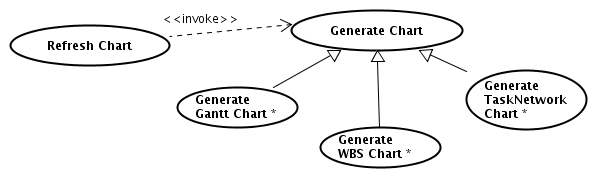
\includegraphics[width=0.7\textwidth]{desing_spec/GenerateChart.png}
\caption{spaccato tratto dal package \emph{Commons} del documento di analisi,
parte \emph{Use cases}}

\end{figure}
Verranno testati tutti gli use case espressi dalla figura tranne ``Refresh
Chart'' in quanto \`e stato riportato solo per favorire la comprensione del
contesto e perche la sua attivit\`a di costruire la \emph{UserOptionChoice} e
recuperare l'insieme dei \emph{Task} vengono testate nel documento
\footnote{make a test document for these use cases.}

\section{Raffinamento della strategia}
\begin{description}
  \item[costruzione strutture di input] Gli usi case descritti nella sezione 
\ref{sec:GenerateChart}, verranno testati usando come input strutture valide e
strutture non valide. Le strutture di input (sia valide che non) verranno
definite in modo che lo use case venga esercitato per la generazione dei
dettagli descritti nel documento di analisi e cercare di provare la generazione
di gran parte delle notazioni grafiche (relative al tipo \emph{Chart} che si
sta considerando).
  \item[confronto dell'output] Per ogni use case di ``generazione'' verranno 
  prodotti dei modelli, in notazione \emph{mockup} disegnati a mano, per poter 
  effettuare il confronto con le immagini di output generate
  dall'implementazione.
  \item[modalit\`a di esecuzione] Ogni use case verr\`a esercitato in modo 
  \emph{individuale}, non verranno esercitate combinazioni con altri use case,
  come la figura esprime.
\end{description}

\section{Tests identification}
\label{sec:GenerateChartTestIdentification}
\footnote{per ogni subsection put the reference to the relative case
specification}
\begin{description}
  \item[gantt]
  \item[wbs]
  \item[task network] 
\end{description}

\section{Pass/fail criteria}
Il risultato di questo desing \`e
espresso dalla seguente relazione rappresentata da questa tabella: 
\begin{table}[h!]
  \begin{center}
    \begin{tabular}{| l | l |}
    \hline
    \textbf{risultato} & \textbf{criteri} \\
	\hline    
	success & numero di \emph{minor} failures $\leq 5$   \\
    \hline
    \emph{minor} failure & numero di \emph{minor} failures $> 5$ \\
    \hline
    \emph{critical} failure & almeno una \emph{critical} failure \\
    \hline
    \emph{blocking} failure & almeno una \emph{blocking} failure \\
    \hline
    \end{tabular}
  \end{center}
	\caption{La colonna \emph{criteri} si riferisce all'insieme di tests 
	identificati nella sezione \ref{sec:GenerateChartTestIdentification}}
\end{table}
